\documentclass[12pt]{article}
        \makeatletter
        \def\input@path{{../../}}
        \makeatother
        \usepackage{sbc-template}
        \makeatletter
        \renewcommand{\inst}[1]{}
        \makeatother
        \usepackage{graphicx,url}
        \usepackage[utf8]{inputenc}
        \usepackage[T1]{fontenc}
        \usepackage[brazil]{babel}
        \usepackage{longtable,booktabs,array}
        \usepackage{amsmath,amssymb}
        \providecommand{\tightlist}{%%
          \setlength{\itemsep}{0pt}\setlength{\parskip}{0pt}}
        \sloppy
        \title{Fundamentos de Reservoir Computing: da intuicao ao modelo minimo}
        \author{}
        \address{}
        \begin{document}

        \maketitle

        \begin{resumo}
        Este artigo apresenta Reservoir Computing (RC) como o primeiro grande degrau teorico da serie. O foco nao e apenas definir o termo, mas mostrar como um reservatorio transforma uma sequencia de entradas em uma representacao dinamica rica e por que isso e util em previsao temporal. Partimos da intuicao de memoria distribuida, formalizamos o modelo minimo com equacoes, conectamos cada elemento do formalismo a arquivos reais do projeto e mostramos artefatos computacionais intermediarios do caso Favorita. Ao final, o leitor consegue ler o codigo do RC classico do projeto, entende o papel do \texttt{washout}, sabe o que e treinado e o que nao e treinado e fica preparado para executar o primeiro pipeline completo no artigo seguinte.
        \end{resumo}

        \subsection{1. O que o leitor vai aprender}\label{1-o-que-o-leitor-vai-aprender}

Ao final deste artigo, voce sera capaz de:

\begin{enumerate}
\def\labelenumi{\arabic{enumi}.}
\tightlist
\item
  definir um reservatorio classico de forma matematica;
\item
  distinguir estado interno, vetor de entrada e readout;
\item
  explicar o papel de \texttt{spectral\_radius}, \texttt{leak\_rate} e \texttt{washout};
\item
  mapear as equacoes de RC para a implementacao em \texttt{code/rc/model.py};
\item
  interpretar artefatos intermediarios, e nao apenas metricas finais.
\end{enumerate}

\subsection{2. A intuicao: um reservatorio e uma memoria dinamica}\label{2-a-intuicao-um-reservatorio-e-uma-memoria-dinamica}

Em um modelo tabular tradicional, as features costumam ser calculadas explicitamente: lags, medias moveis, indicadores de calendario e assim por diante. Em RC, a ideia e diferente. Em vez de escrever manualmente toda a representacao temporal, injetamos a sequencia em um sistema dinamico recorrente e usamos seus estados internos como uma base de representacao.

A intuicao mais util para iniciantes e esta:

\begin{itemize}
\tightlist
\item
  a entrada \(u_t\) perturba o sistema;
\item
  o estado \(x_t\) carrega um resumo dinamico do passado recente;
\item
  o readout linear aprende a converter esse resumo em previsao.
\end{itemize}

RC e atraente didaticamente porque separa o problema em duas partes:

\begin{enumerate}
\def\labelenumi{\arabic{enumi}.}
\tightlist
\item
  um mecanismo fixo de representacao temporal;
\item
  uma camada simples de regressao treinavel.
\end{enumerate}

\subsection{3. O modelo minimo de RC}\label{3-o-modelo-minimo-de-rc}

No projeto, o reservatorio classico e implementado com a seguinte dinamica:

\[
x_t = (1 - \alpha) x_{t-1} + \alpha \tanh(W_{res} x_{t-1} + W_{in} u_t + b),
\]

em que:

\begin{itemize}
\tightlist
\item
  \(u_t \in \mathbb{R}^d\) e o vetor de entrada no tempo \(t\);
\item
  \(x_t \in \mathbb{R}^N\) e o estado do reservatorio;
\item
  \(W_{res}\) e a matriz recorrente interna;
\item
  \(W_{in}\) projeta a entrada para o espaco do reservatorio;
\item
  \(b\) e um vetor de bias;
\item
  \(\alpha\) e o \texttt{leak\_rate}.
\end{itemize}

No codigo, isso aparece em \texttt{EchoStateReservoir.step()}:

\begin{verbatim}
pre_activation = (
    self.recurrent_weights @ self.state
    + self.input_weights @ input_vector
    + self.bias
)
new_state = np.tanh(pre_activation)
self.state = (1.0 - self.config.leak_rate) * self.state + self.config.leak_rate * new_state
\end{verbatim}

A previsao e feita por um readout linear:

\[
\hat{y}_t = W_{out} \phi_t,
\qquad
\phi_t = [1; u_t; x_t].
\]

No projeto, \texttt{\textbackslash{}phi\_t} e construida por \texttt{\_feature\_vector()} e \texttt{W\_out} e ajustado via regressao Ridge.

\subsection{4. O que e treinado e o que nao e treinado}\label{4-o-que-e-treinado-e-o-que-nao-e-treinado}

Um dos pontos mais didaticos de RC e a divisao entre dinamica fixa e leitura treinavel.

No projeto:

\begin{itemize}
\tightlist
\item
  \texttt{W\_in}, \texttt{W\_res} e \texttt{b} sao inicializados aleatoriamente e mantidos fixos;
\item
  apenas o readout linear e ajustado com supervisao.
\end{itemize}

Formalmente, o treinamento resolve

\[
W_{out}^* = \arg\min_{W_{out}}
\|Y - \Phi W_{out}\|_2^2 + \lambda \|W_{out}\|_2^2,
\]

em que \(\Phi\) e a matriz de features acumuladas ao longo do tempo e \(\lambda\) e o hiperparametro de regularizacao Ridge.

Essa escolha reduz o custo de treinamento em relacao a RNNs totalmente treinaveis e, ao mesmo tempo, preserva uma representacao temporal rica.

\subsection{5. Como o tempo entra no modelo}\label{5-como-o-tempo-entra-no-modelo}

No projeto, o vetor de entrada sequencial e construindo em \texttt{code/common/sequential\_features.py} com sete componentes:

\begin{itemize}
\tightlist
\item
  demanda previa normalizada;
\item
  promocao normalizada;
\item
  \texttt{dow\_sin}, \texttt{dow\_cos};
\item
  \texttt{month\_sin}, \texttt{month\_cos};
\item
  indicador de fim de semana.
\end{itemize}

Em notacao compacta,

\[
u_t =
\begin{bmatrix}
\widetilde{y}_{t-1} &
\widetilde{p}_t &
\sin(2\pi \, \mathrm{dow}_t / 7) &
\cos(2\pi \, \mathrm{dow}_t / 7) &
\sin(2\pi \, \mathrm{month}_t / 12) &
\cos(2\pi \, \mathrm{month}_t / 12) &
\mathbb{1}_{\mathrm{weekend}}
\end{bmatrix}^\top.
\]

Esse vetor coloca em uma mesma representacao:

\begin{itemize}
\tightlist
\item
  memoria de curtissimo prazo, via \(\widetilde{y}_{t-1}\);
\item
  contexto exogeno, via promocao;
\item
  ciclo temporal, via senos e cossenos.
\end{itemize}

\subsection{6. O papel do washout}\label{6-o-papel-do-washout}

Nos primeiros instantes da simulacao, o estado do reservatorio ainda esta fortemente contaminado pela inicializacao. Por isso, o projeto descarta os primeiros passos antes de treinar o readout.

Se chamarmos o \texttt{washout} de \(w\), o treino do readout usa apenas os tempos \(t \ge w\):

\[
\Phi = [\phi_w, \phi_{w+1}, \dots, \phi_T]^\top.
\]

Em \texttt{fit\_rc\_readout()}, isso aparece no teste \texttt{if\ idx\ \textgreater{}=\ config.washout}.

O \texttt{washout} nao e um detalhe de implementacao. Ele e uma parte conceitual do pipeline, porque separa a transiente inicial da dinamica que realmente queremos aproveitar.

\subsection{7. Como o projeto implementa RC no caso Favorita}\label{7-como-o-projeto-implementa-rc-no-caso-favorita}

A tabela abaixo resume o pipeline implementado.

\begin{longtable}[]{@{}lll@{}}
\toprule\noalign{}
Objeto & Dimensao no projeto & Origem \\
\midrule\noalign{}
\endhead
\bottomrule\noalign{}
\endlastfoot
Vetor de entrada \(u_t\) & 7 & \texttt{scaled\_input\_vector()} \\
Estado do reservatorio \(x_t\) & 80 & \texttt{RCConfig.n\_reservoir} \\
Vetor de features \([1; u_t; x_t]\) & 88 & \texttt{\_feature\_vector()} \\
Readout & 1 saida & Ridge linear sobre as features \\
\end{longtable}

O fluxo completo do codigo e o seguinte:

\begin{enumerate}
\def\labelenumi{\arabic{enumi}.}
\tightlist
\item
  \texttt{build\_scaler\_state()} calcula medias e desvios para normalizacao;
\item
  \texttt{scaled\_input\_vector()} construi \(u_t\);
\item
  \texttt{EchoStateReservoir.step()} atualiza \(x_t\);
\item
  \texttt{\_feature\_vector()} monta \(\phi_t = [1; u_t; x_t]\);
\item
  \texttt{Ridge.fit()} estima o readout;
\item
  \texttt{forecast\_rc()} faz previsao recursiva no bloco de teste.
\end{enumerate}

O trecho central do treinamento e este:

\begin{verbatim}
input_vector = scaled_input_vector(prev_y, row, scaler=scaler)
state = reservoir.step(input_vector)
feature_rows.append(_feature_vector(state, input_vector))
targets.append(float(row["y"]))
\end{verbatim}

Isso mostra a ideia central de RC em sua forma mais simples: o modelo nao aprende uma representacao temporal diretamente por backpropagation; ele coleta estados dinamicos e aprende apenas como le-los.

\subsection{8. O que os artefatos intermediarios mostram}\label{8-o-que-os-artefatos-intermediarios-mostram}

O artigo nao precisa esperar a metrica final para ensinar alguma coisa. Os artefatos computacionais deste modulo mostram o pipeline em um nivel mais interno.

\pandocbounded{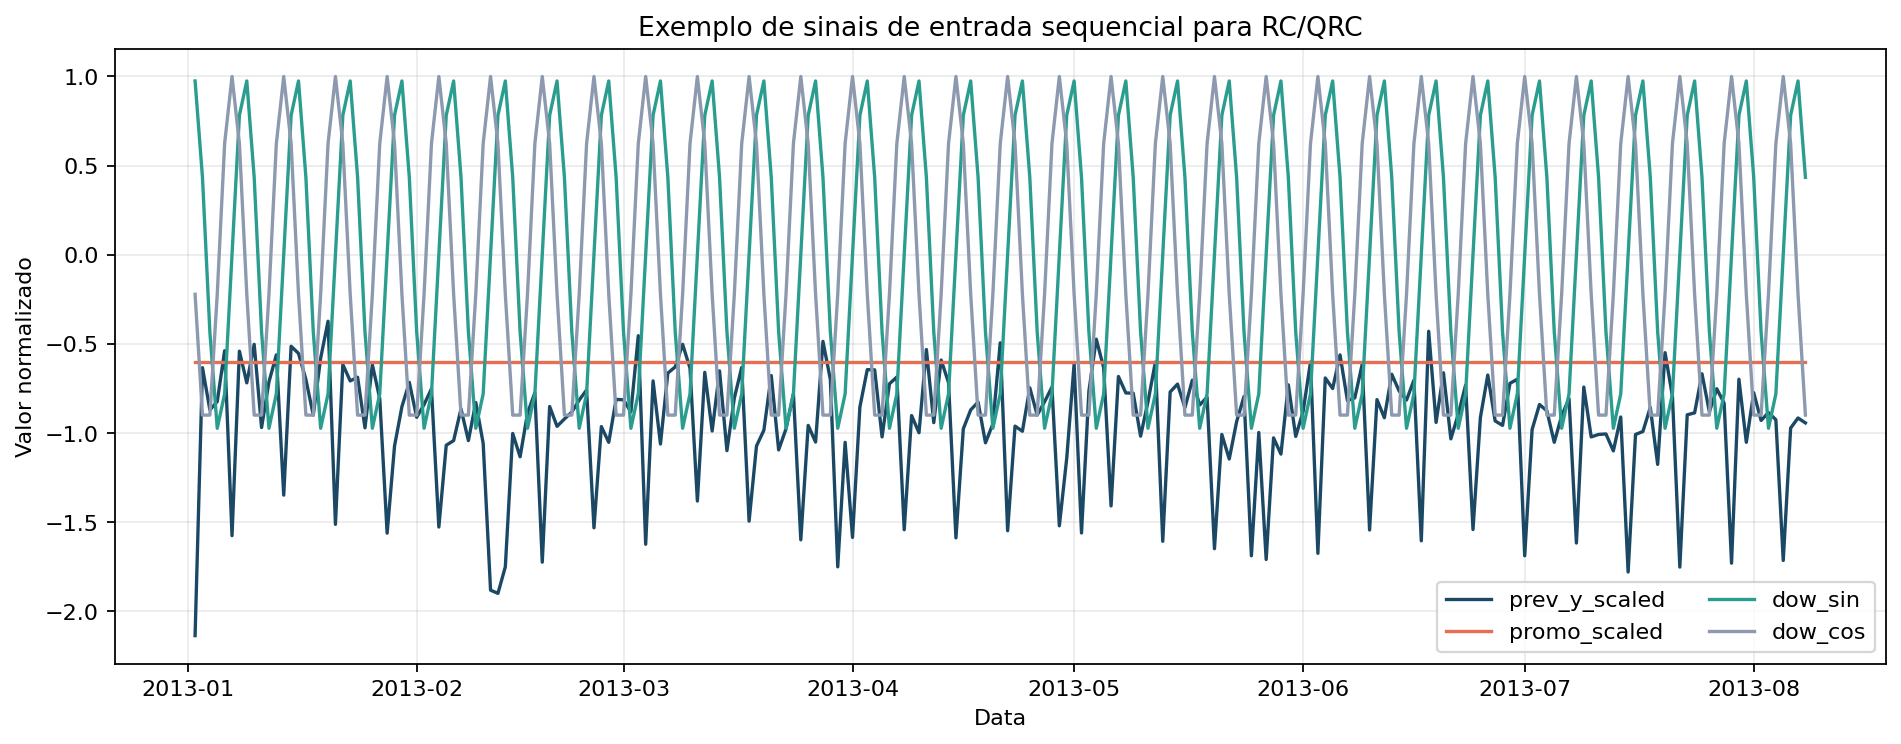
\includegraphics[keepaspectratio,alt={Exemplo dos sinais de entrada sequenciais usados pelo RC.}]{computational_results_20260402_222902/sequential_inputs_example.png}}

A imagem de entrada sequencial mostra que o reservatorio nao recebe apenas uma serie de vendas crua. Ele recebe uma codificacao temporal e exogena compacta.

\pandocbounded{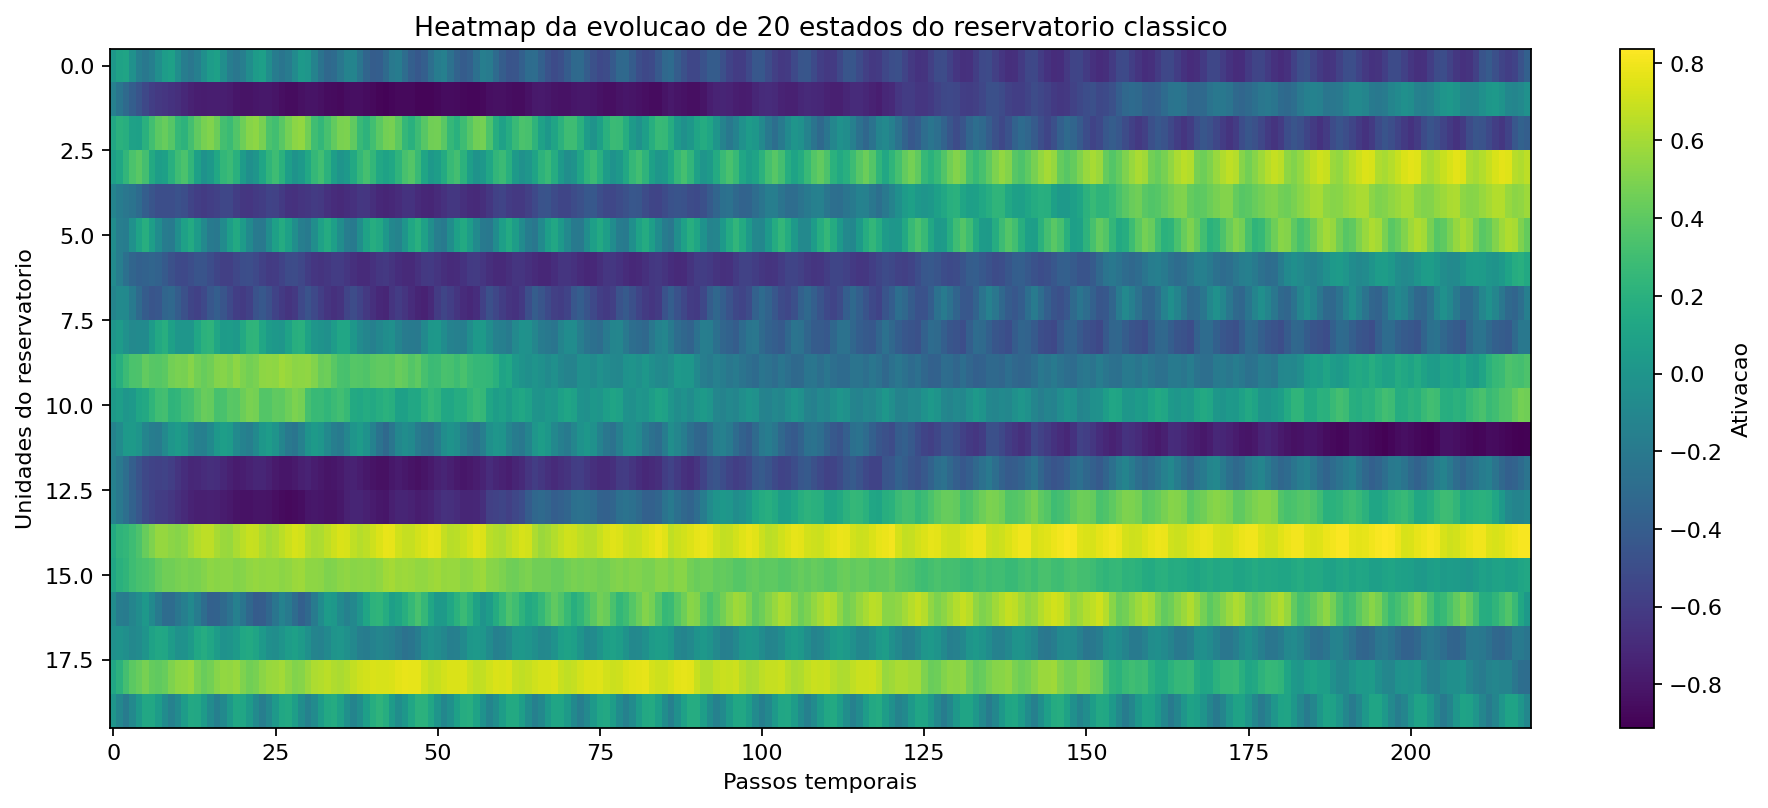
\includegraphics[keepaspectratio,alt={Heatmap dos estados internos do reservatorio classico no recorte Favorita.}]{computational_results_20260402_222902/rc_state_heatmap.png}}

O heatmap dos estados ilustra duas ideias importantes:

\begin{enumerate}
\def\labelenumi{\arabic{enumi}.}
\tightlist
\item
  unidades diferentes respondem de modos diferentes ao mesmo estimulo;
\item
  a memoria do reservatorio nao e um unico lag explicito, mas uma combinacao distribuida de estados.
\end{enumerate}

Em outras palavras, RC construi uma base dinamica de features sem precisar enumerar manualmente toda a interacao temporal.

\subsection{9. Comparando RC com outras familias de modelo}\label{9-comparando-rc-com-outras-familias-de-modelo}

Vale situar RC entre outros paradigmas que tambem aparecem na serie:

\begin{itemize}
\tightlist
\item
  \texttt{Seasonal\ Naive}, \texttt{ETS} e \texttt{Prophet} modelam estrutura temporal de forma mais explicita;
\item
  \texttt{XGBoost} usa engenharia de atributos tabulares;
\item
  \texttt{LSTM} aprende dinamica recorrente via gradiente;
\item
  \texttt{RC} fixa a dinamica recorrente e treina apenas o readout.
\end{itemize}

Essa posicao intermediaria e pedagogicamente muito poderosa. RC e mais rico do que um baseline ingenuo, mas muito mais simples de treinar do que uma RNN completa.

\subsection{10. Passo-a-passo para estudar ou modificar o RC do projeto}\label{10-passo-a-passo-para-estudar-ou-modificar-o-rc-do-projeto}

Um leitor que queira estudar a implementacao deve seguir esta ordem:

\begin{enumerate}
\def\labelenumi{\arabic{enumi}.}
\tightlist
\item
  abrir \texttt{code/common/sequential\_features.py};
\item
  verificar como o vetor \texttt{u\_t} e construindo;
\item
  abrir \texttt{code/rc/model.py} e localizar \texttt{RCConfig};
\item
  ler \texttt{EchoStateReservoir.step()} junto da equacao do artigo;
\item
  ler \texttt{fit\_rc\_readout()} e localizar o \texttt{washout};
\item
  executar \texttt{python\ code/rc/run.py};
\item
  validar o comportamento com \texttt{pytest\ code/rc/test\_model.py}.
\end{enumerate}

Essa ordem importa. Se o leitor abrir apenas \texttt{run.py}, perde a correspondencia entre teoria e implementacao.

\subsection{11. Conclusao}\label{11-conclusao}

RC ja esta completamente formulado no contexto do projeto. Temos uma definicao matematica, uma implementacao concreta e artefatos intermediarios que mostram a representacao temporal em acao. O proximo passo natural e colocar esse modelo em confronto com um baseline forte, medindo o que ele realmente entrega no recorte Favorita.

\subsection{Entregaveis associados no repositorio}\label{entregaveis-associados-no-repositorio}

\begin{itemize}
\tightlist
\item
  implementacao do RC: \texttt{code/rc/model.py}
\item
  execucao do RC: \texttt{code/rc/run.py}
\item
  testes do RC: \texttt{code/rc/test\_model.py}
\item
  construcao de entrada sequencial: \texttt{code/common/sequential\_features.py}
\item
  artefatos deste artigo: \texttt{computational\_results\_20260402\_222902/}
\end{itemize}

\subsection{Referencias}\label{referencias}

\begin{itemize}
\tightlist
\item
  Jaeger, H. The "echo state" approach to analysing and training recurrent neural networks.
\item
  Lukosevicius, M.; Jaeger, H. Reservoir computing approaches to recurrent neural network training.
\item
  Luko sevicius, M. A practical guide to applying echo state networks.
\item
  Fujii, K.; Nakajima, K. Harnessing disordered-ensemble quantum dynamics for machine learning.
\end{itemize}

        \end{document}
